\subsection{Class Diagram}
In the RASD document a Class Diagram has been showed to model the problem, including all the classes involved without going into too much detail.\\
For this reason, in this section an updated Class Diagram is introduced to represent the system from an  implementation oriented point of view. \\

The following diagram differs from the one presented in the RASD in two aspects:
\begin{itemize}
    \item the main methods of each kind of user are presented;
    \item attributes data types are specified.
\end{itemize}

\begin{figure}[H]
  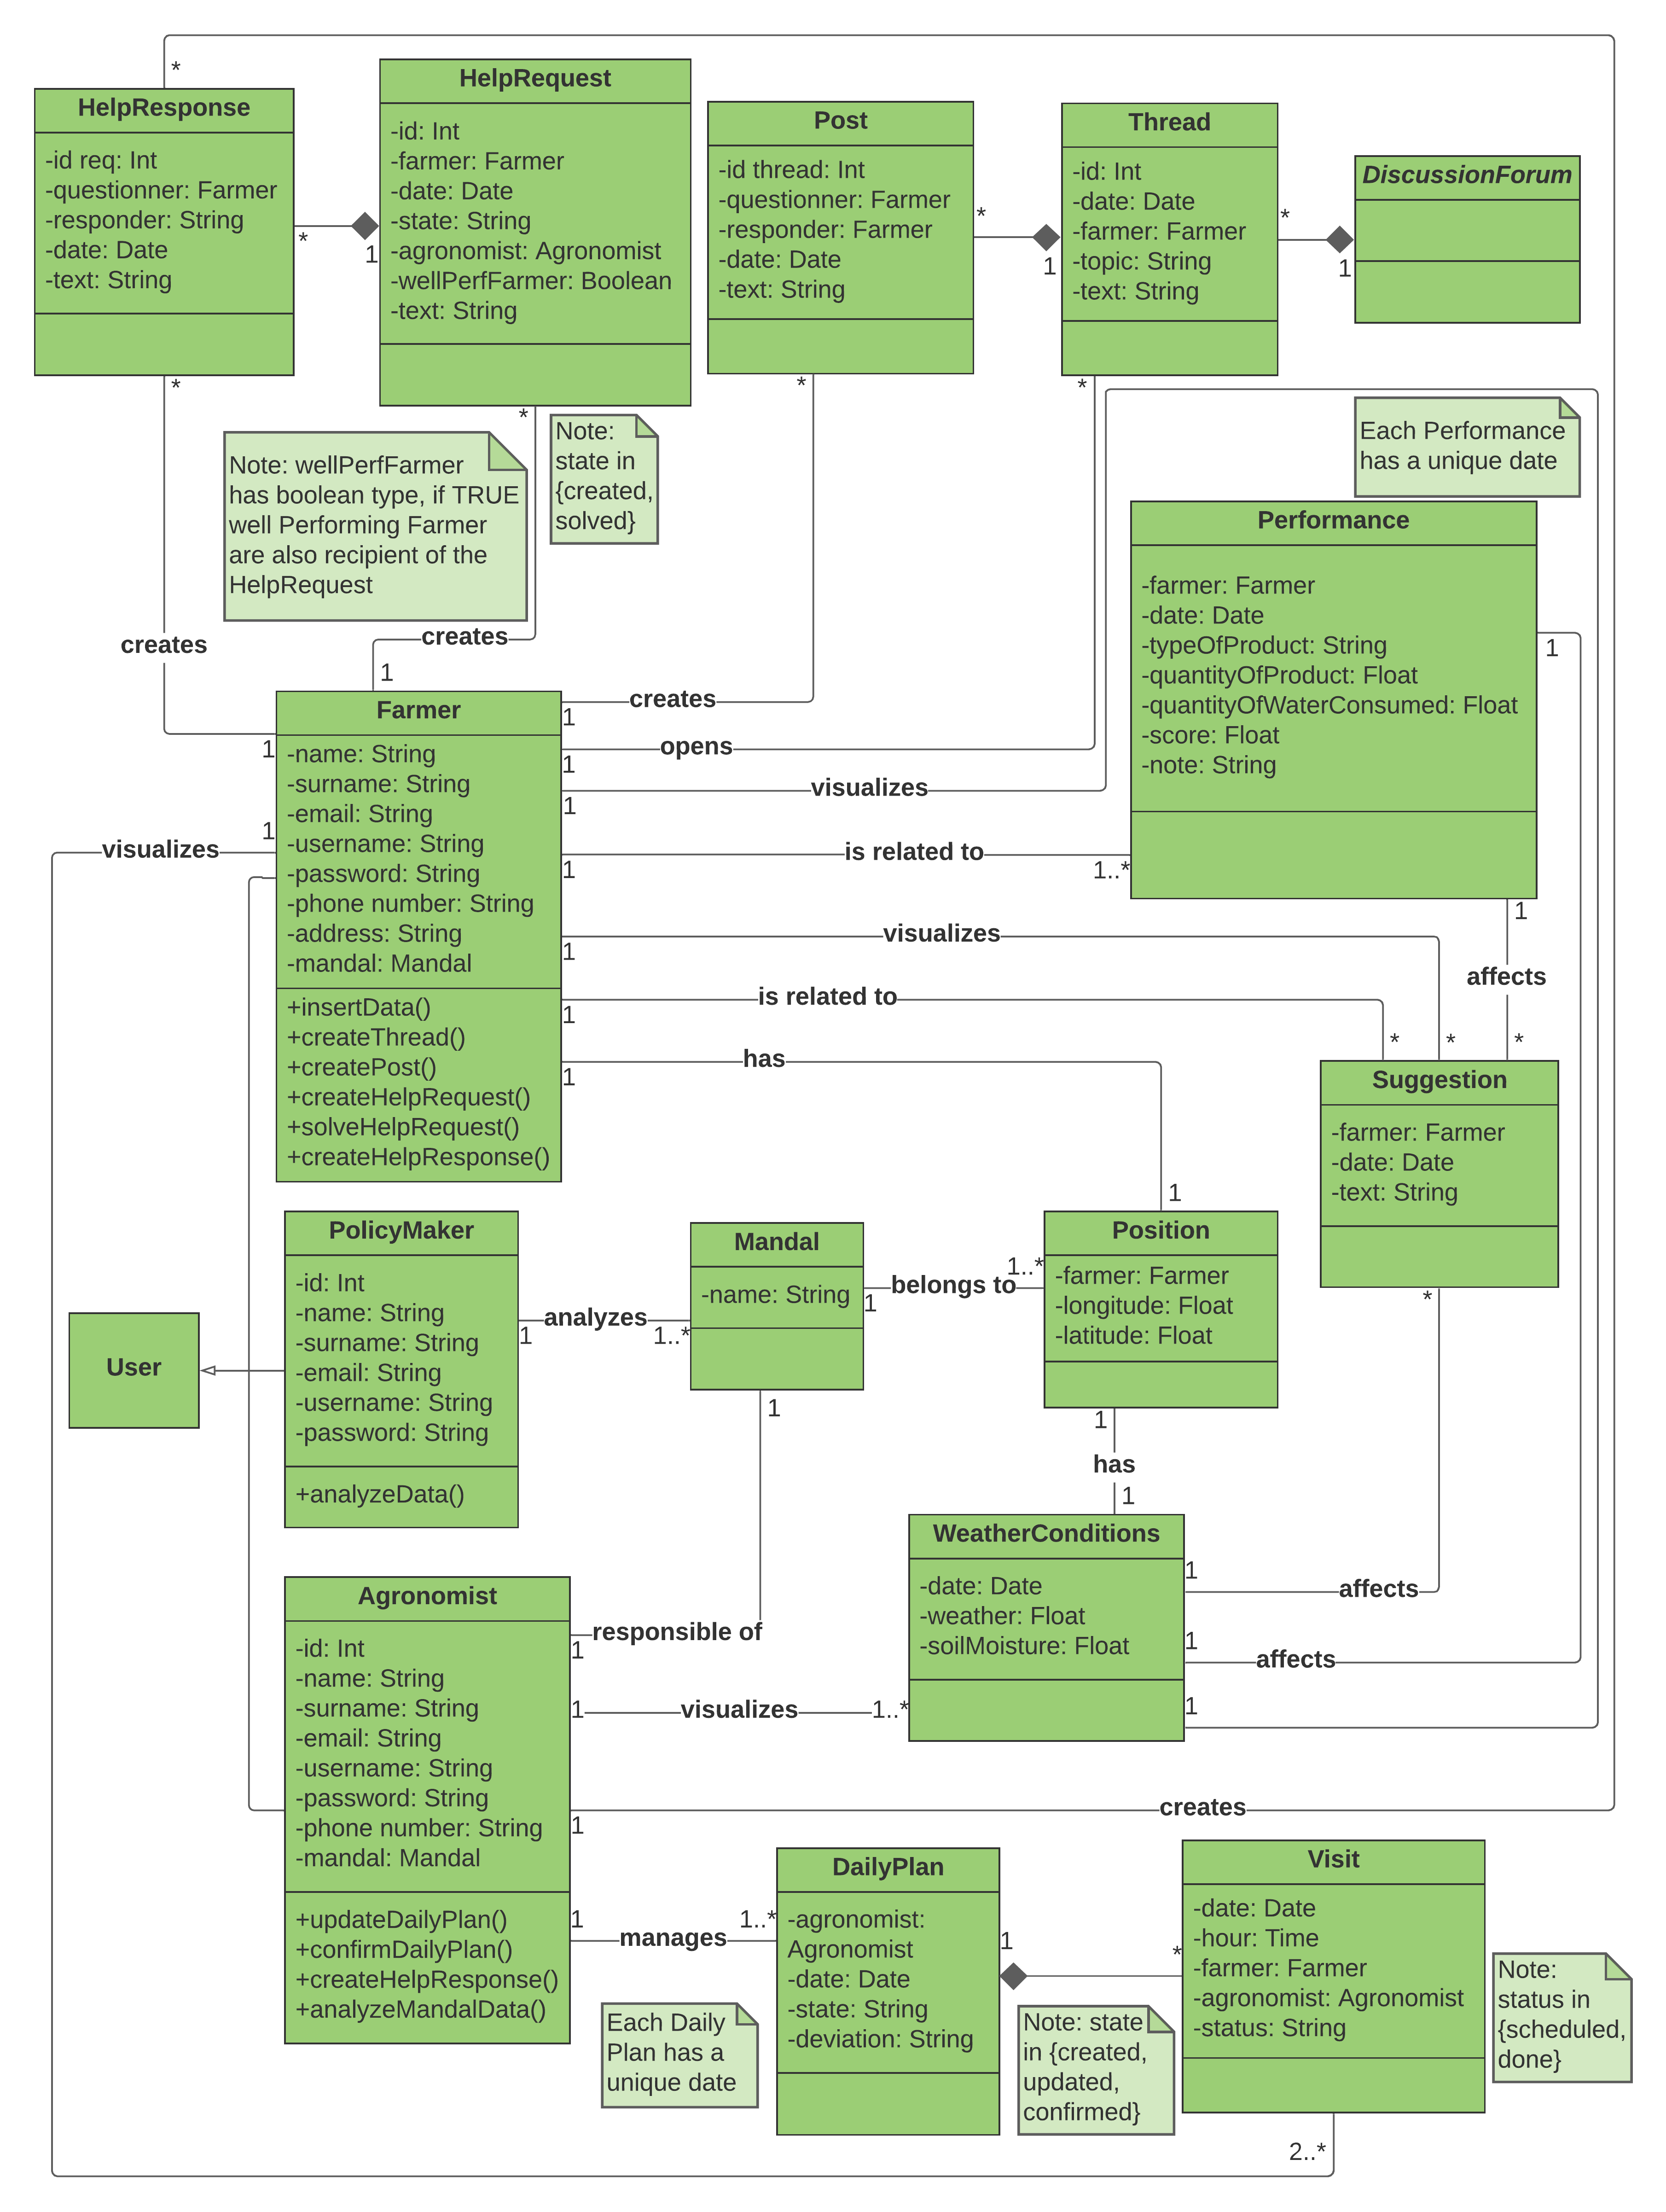
\includegraphics[width=125.5mm,scale=0.9]{./Images/Class Diagram.png}
  \caption{Class Diagram}
\end{figure}